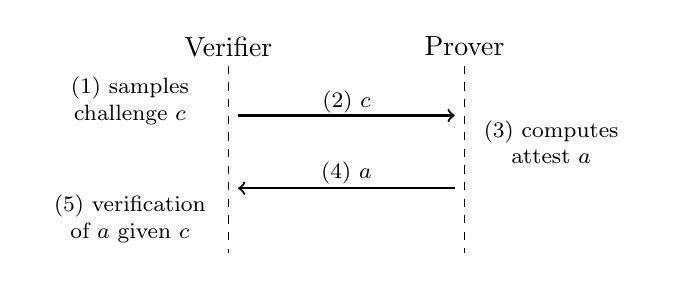
\begin{tikzpicture}[
	squarednode/.style={rectangle, draw=black, thick, minimum size=10mm},
	invisiblenode/.style={rectangle, draw=white}
]
	%Nodes
	\node (verifier) at (0.5,2) {Verifier};
	\node[invisiblenode] (1) at (0.5,1) {};
	\node[invisiblenode] (2) at (0.5,0.2) {};
	\node[invisiblenode] (3) at (0.5,-.75) {};
	
	\node (prover) at (3.5,2) {Prover};
	\node[invisiblenode] (4) at (3.5,1) {};
	\node[invisiblenode] (5) at (3.5,0.2) {};
	\node[invisiblenode] (6) at (3.5,-.75) {};
	
	\node[invisiblenode](sample) at (-0.75,1.3) 
		   {\footnotesize\begin{tabular}{c}(1) samples \\challenge $c$\end{tabular}};
		   \node[invisiblenode](nonce) at (2,1.3) 
		        {\footnotesize(2) $\boldsymbol{c}$};
		        \node[invisiblenode](attest) at (4.6,.75) 
		             {\footnotesize\begin{tabular}{c} (3) computes \\ attest $\boldsymbol{a}$ \end{tabular}};
		             \node[invisiblenode](reply) at (2,0.4) 
		                  {\footnotesize(4) $\boldsymbol{a}$};
		                  \node[invisiblenode](verify) at (-0.75,-0.2)
		                       {\footnotesize\begin{tabular}{c} (5) verification \\ of $\boldsymbol{a}$ given $\boldsymbol{c}$ \end{tabular}};
		                       
		                       %Lines
		                       \draw[dashed]    (verifier.south) -- (3.north);
		                       \draw[dashed]    (prover.south)   -- (6.north);
		                       \draw[->, thick] (1.north east)   -- (4.north west);
		                       \draw[<-, thick] (2.east)         -- (5.west);
		                       
\end{tikzpicture}


